\documentclass{article}
\usepackage[utf8]{inputenc}
\usepackage[a4paper, total={6in, 8in}]{geometry}
\usepackage{graphicx}
\usepackage{caption}
\usepackage{subcaption}
\usepackage{commath}
\usepackage{mathrsfs,amsmath}


\usepackage{listings}
\usepackage{color} 

\usepackage[linkbordercolor={0 0 1}]{hyperref}
\hypersetup{
    colorlinks,
    citecolor=black,
    filecolor=black,
    linkcolor=black,
    urlcolor=black
}


\begin{document}

\begin{titlepage}

\newcommand{\HRule}{\rule{\linewidth}{1mm}} 
\center 

\textsc{\LARGE Ecole Polytechnique Fédérale de Lausanne}\\[1.5cm]
\textsc{\Large Bachelor Project}\\[0.5cm]  

\HRule \\[0.4cm]
{ \huge \bfseries ApiZoom – deep learning to quantify the Varroa parasite in honey bee hive images}\\[0.4cm] 
\HRule \\[1.5cm]


\begin{minipage}{0.4\textwidth}
\begin{flushleft} \large
\emph{Author:}\\
Joe \textsc{Najm}\\
\emph{Sciper:} 301560
\end{flushleft}
\end{minipage}
~
\begin{minipage}{0.4\textwidth}
\begin{flushright} \large
\emph{Supervisors:} \\
Prof. Jean-Philippe \textsc{Thiran} \\
Roser \textsc{Vinals Terres} \\
\end{flushright}
\end{minipage}\\[1cm]


{\large 8 credits}\\
{\large Spring 2021}\\[1cm] 


\includegraphics[scale = 0.4]{epfl.png}\\[1cm]

\vfill

\end{titlepage}



\newpage


\begin{abstract}

    Detecting and counting the number of varroa mites that infected a hive is crucial. This task has been traditionally done by counting manually the number of varroa mites. However, a new tool called ApiZoom based on deep learning has allowed to automatise the counting of varroa mites from an image. Recently, the network used by ApiZoom has been upgraded to YOLOv5, which has shown a huge potential for detecting varroa mites. Nevertheless, the results were obtained without optimising the hyperparameters of the network. Furthermore, the website used for annotating the images   did not allow the admin user to manually modify the bounding boxes and annotations on a prediction made by the network on the website, giving rise to inaccurate labels that were used for training. Thus, this project tackles both issues. First, we will evolve the hyperparameters in an attempt to obtain better detection results from the network. We will prove that optimising the hyperparameters can led to some improvement although not significant.  Second,  we will implement new features on the website allowing the admin user to manually adjust the position and size of a prediction in order to improve the accuracy of the training images fed to the network.
    
    
\end{abstract}

\newpage

\tableofcontents
\vfill


\newpage
\section{Introduction}

\subsection{The Varroa Mite : Coronavirus of bees}

It is widely known that bees are one of the most important insects on earth : not only do they provide us with honey, they are also a key factor in the pollination of flowers and fruits. Although bees are still not on the endangered animals list, their population is dropping at a worrying rate. One of the key factors for that drop is the Varroa Mite (\hyperref[Figure 1]{Figure 1}), a parasite originally from Asia that reached Switzerland in 1984. 

\begin{figure}[!ht]
  \centering
  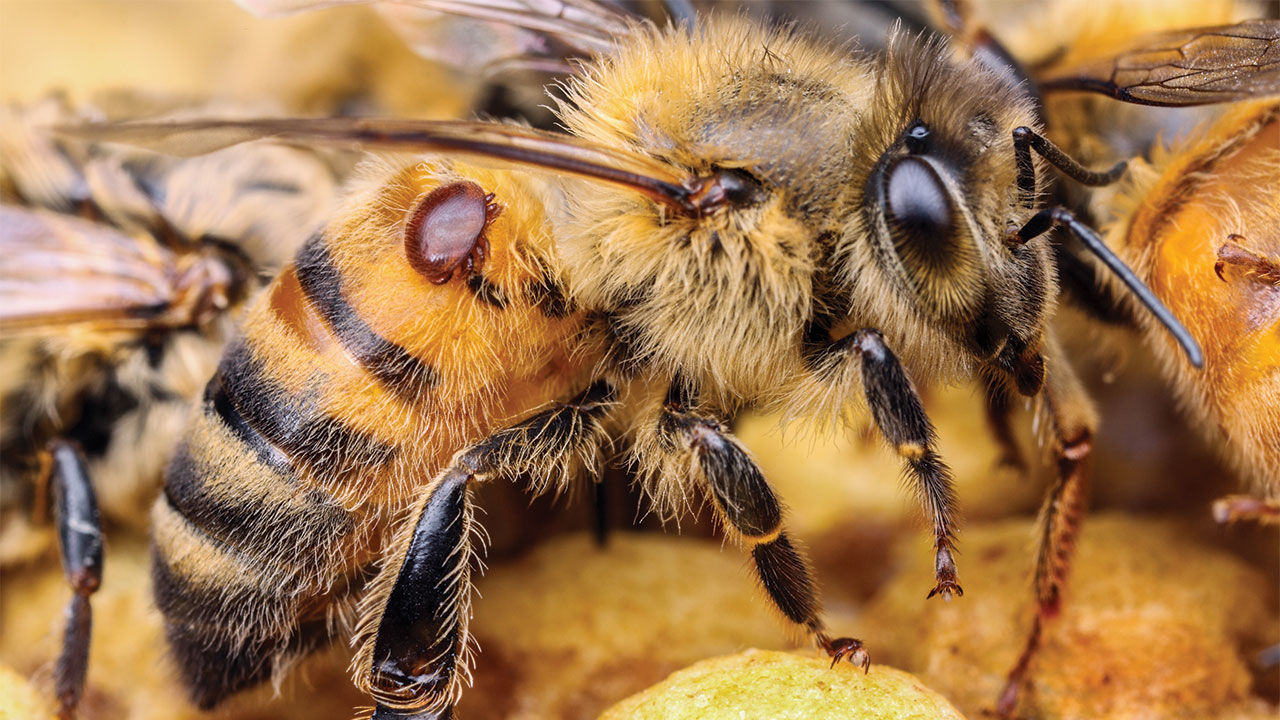
\includegraphics[scale = 0.20]{Bees/varroa.jpg}
  \caption{Varroa mite on a bee}
  \label{Figure 1}
\end{figure}

It will stick on a bee, once the bee goes back to its hive, it will drop to the bottom of the hive, and infect the larvas (\hyperref[Figure 2]{Figure 2}) by feeding off them and laying eggs in them. The  new born bee will be weaker and more vulnerable to other deceases. If not treated correctly and on time, a varroa infection can wipe out an entire colony in less than 3 years, therefore it is really important for beekeepers to react fast once an infection was spotted. 

\begin{figure}[!ht]
  \centering
  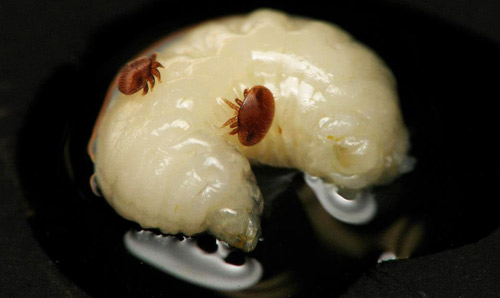
\includegraphics[scale = 0.5]{Bees/larvae.jpg}
  \caption{Varroa mite on a bee larvae}
  \label{Figure 2}
\end{figure}


\subsection{An archaic solution}
To evaluate the hive's health, beekeepers place a board under the hive (\hyperref[Figure 3]{Figure 3}) and count by hand the number of dead varroa. This method is very laborious as the varroa mites are really small (1–1.8 mm long and 1.5–2 mm wide) and could be highly inaccurate for amateur beekeepers as the board will also be full of debris. 

\begin{figure}[!ht]
  \centering
  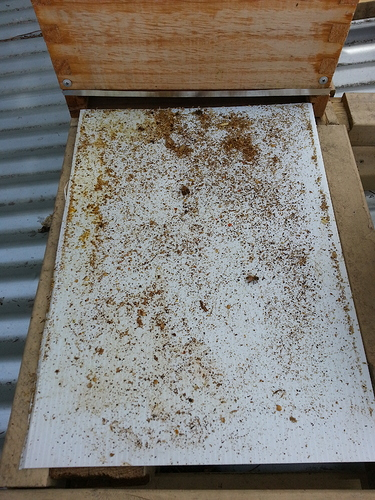
\includegraphics[scale = 0.5]{Bees/board.jpg}
  \caption{Bottom board of a hive}
  \label{Figure 3}
\end{figure}

\subsection{Objectives of the project}

ApiZoom is a Deep Learning model based on YOLOv5 that detects mites from the picture of a board.
It contains three main aspects (\hyperref[Figure 4]{Figure 4}): Deep Learning that will generate the detection network, Website where we can use the network on some new images and the database that will contain annotated images (coming from the website) to be used for future training of the Deep Learning network.

\bigskip

The main goal of this project is to improve the Deep Learning model.
To do so, we have defined two specific goals:
1. Improve the performance of the deep learning model by optimising the hyperparameters and data augmentation.
2. Improve the quality of the annotations by allowing the admin user to change the size and position of the bounding boxes in the Apizoom website.

\begin{figure}[!ht]
  \centering
  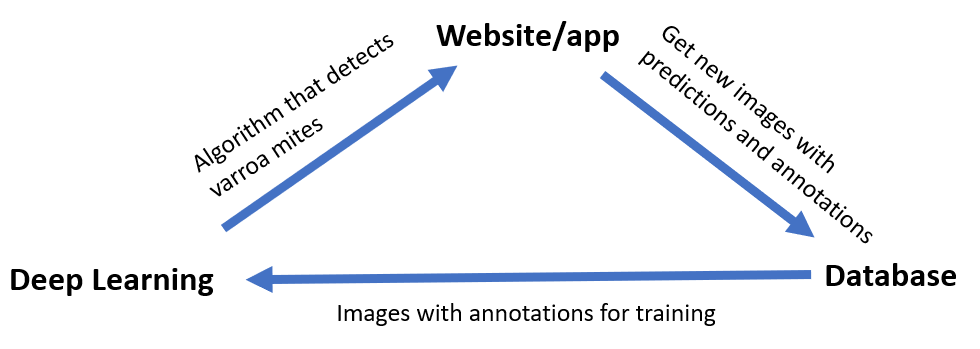
\includegraphics[scale = 0.5]{triangle.png}
  \caption{ApiZoom structure}
  \label{Figure 4}
\end{figure}

\subsection{Organisation of the project}

The rest of the report is organised as follows. Section 2 presents the different Object detection state-of-art techniques such as Faster R-CNN and YOLO.
Section 3 presents the metrics and datasets used in the project.
In Section 4, we will look at the hyperparameters evolution results. Lastly in Section 5, we will see the improvement made on the website.  




\newpage
\section{Object detection state-of-art techniques}

\subsection{First image recognition technique}

The first image recognition technique was the "histograms of oriented gradients" (HOG) ~\cite{dalal2005histograms} : we would compute the gradient at each pixel and determine its angle. Depending on the angle, we would draw a histogram with a bin of pre-defined angles and transform this histogram to a 1D structure. This method was particularly used for human recognition. Let's take a look at an example : 

Let's consider a 64*128 image, we divide the image into 7*15 = 105 blocks of 50 \% overlap, with each block being 2*2 cells and each cell 8*8 pixels (\hyperref[Figure 5]{Figure 5}). 

\begin{figure}[!ht]
  \centering
  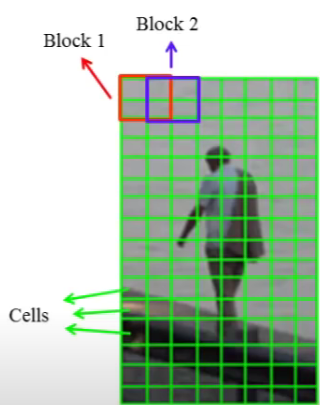
\includegraphics[scale = 1.15]{HOG/cells.PNG}
  \caption{Image divided in cells}
  \label{Figure 5}
\end{figure}

We  now need to look at the gradient orientation : if for example we have $85^o$, we are between the Bin $70^o$ and Bin $90^o$ (\hyperref[Figure 6]{Figure 6}) with a distance of $15^o$ and $5^o$ respectively. 

\begin{figure}[!ht]
  \centering
  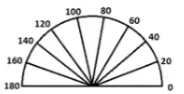
\includegraphics[scale = 2]{HOG/angle_bin.PNG}
  \caption{Bin of angles}
  \label{Figure 6}
\end{figure}

Therefore, the ratios on the histogram are 15/20 = 3/4 and 5/20 = 1/4 at $70^o$ and $90^o$. The histograms are then converted to a 1D matrix and obtain the following (\hyperref[Figure 7]{Figure 7}) :

\begin{figure}[!ht]
  \centering
  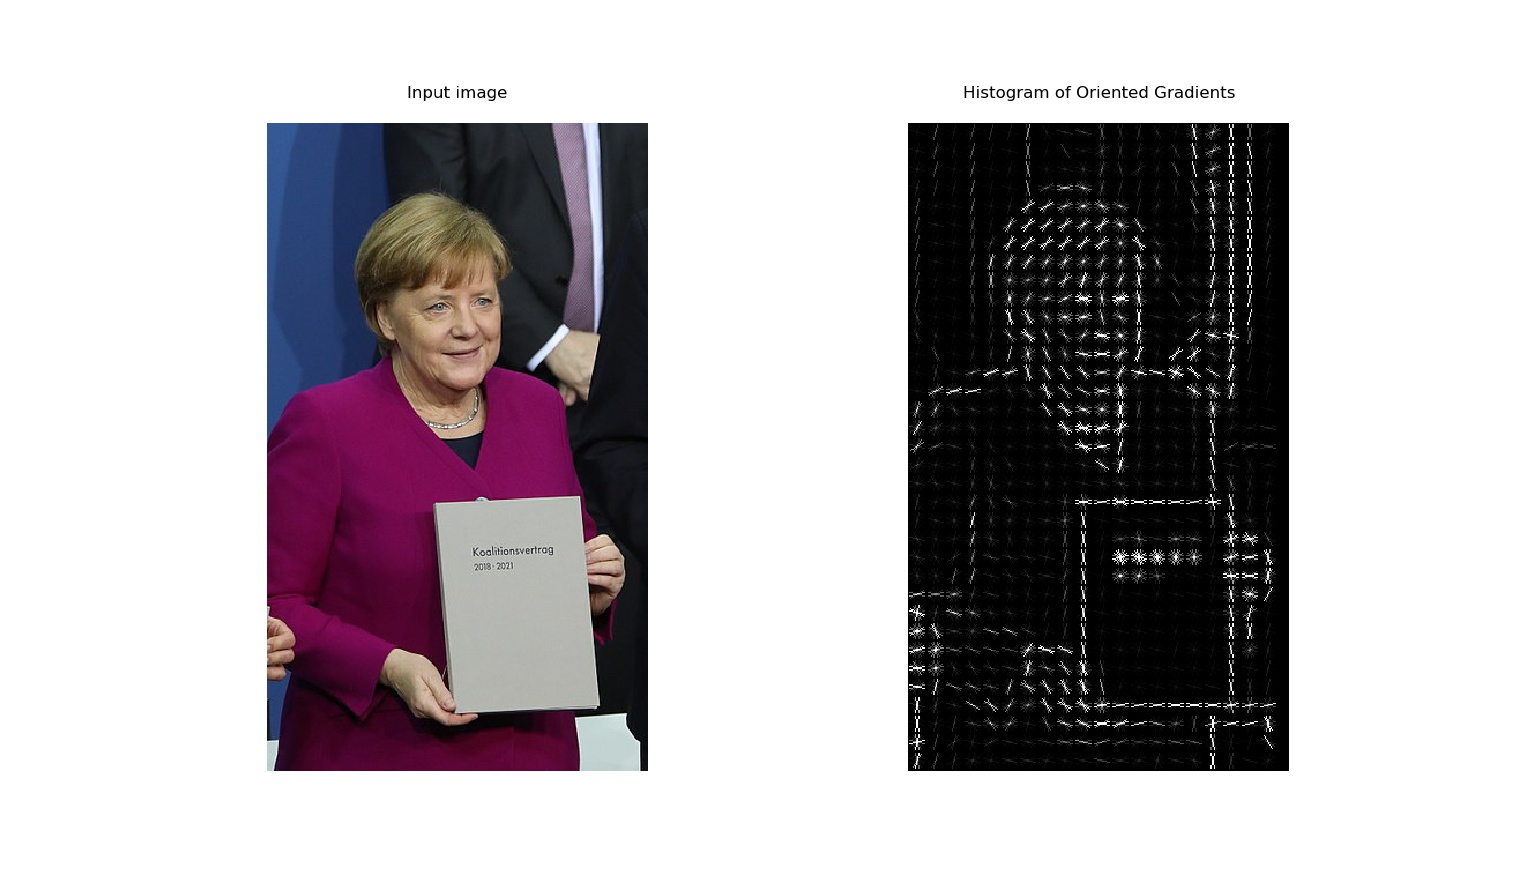
\includegraphics[scale = 0.4]{HOG/example.jpeg}
  \caption{HOG final result}
  \label{Figure 7}
\end{figure}

\newpage
\subsection{Deep learning approaches for object detection}
A more modern approach is to use deep learning and neural networks.
Today, most of the detection techniques rely on Convolutional Neural Network (CNN) to identify objects on an image. It is a succession of multi-dimensional convolutional kernels (filters). We can include pooling in order to reduce the size of the layers. It ends with a fully connected layer in order to apply a classic neural network and find the weights.
We usually want to detect recurrent objects on an image (varroa mites in our case) and indicate their positions with bounding boxes.

\bigskip
\bigskip

Traditionally, 'sliding windows' were used to put the bounding boxes around the objects : a window would slide through the entire image until having the wanted object inside of it and putting a bounding box around it. This method is not efficient at all and was extremely time consuming as we would have to slide through the entire picture. Nowadays, we have much better object detection techniques.

\bigskip
\bigskip

We have 2 main object detection techniques based on CNN : 

\begin{itemize}
    \item One-stage method (YOLO) : we directly detect the objects on the image.
    \item Two-stage method (Faster R-CNN) : we first need to compute a feature map and then we can detect the objects.
\end{itemize}

\bigskip
In the following sections, the structure of these two object detection techniques will be presented.


\subsubsection{Faster R-CNN}

The Faster R-CNN ~\cite{ren2015faster} is a two-stage method, meaning that the convolutional layers will first compute a feature map and then use a Region Proposal Network on the feature map to detect the wanted objects (\hyperref[Figure 8]{Figure 8}). In a nutshell, it will find certain regions of interest and then detect only in those regions by using a sliding window approach (instead of looking at the whole image).

The Faster R-CNN is an improvement of the Fast R-CNN algorithm ~\cite{7410526}. The Fast R-CNN would generate the feature map using a segmentation algorithm, then apply the convolution implementation of sliding windows in the proposed regions. Faster R-CNN uses convolutional layers instead of a segmentation algorithm to find the proposed regions, thus making it much faster.

Unfortunately, the two-stage method is not ideal for real time detection.

\begin{figure}[!ht]
  \centering
  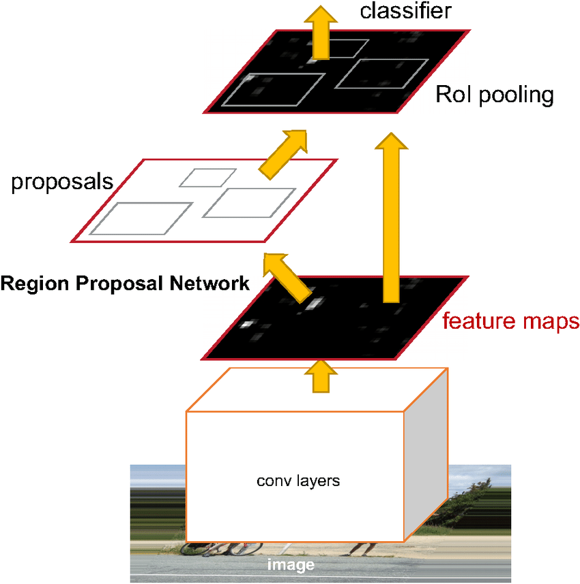
\includegraphics[scale = 0.5]{FastRCNN/faster.png}
  \caption{Faster R-CNN architecture ~\cite{ren2015faster}}
  \label{Figure 8}
\end{figure}


\newpage

\subsubsection{YOLO}

The One-stage method (there is no need to compute a feature map) is much faster than the two-stage method, it is therefore possible to do real time detection. It does not try to find some specific regions of interest on the image, but rather look at it all. This method is more suitable for our varroa detecting algorithm as a varroa is very small and does not occupy a lot of space on the image. Moreover, the parasites are scattered all over the image. Thus we do not really have a specific region of interest on the image where all the varroa mites are located.

\bigskip

Therefore, A more suitable (for this project) algorithm to perform a CNN is the 'You Only Look Once' (YOLO) algorithm ~\cite{redmon2016you}. The name comes from the fact this it does not use sliding windows to detect the objects.

\bigskip

We will first take a look at the first YOLO architecture (\hyperref[Figure 9]{Figure 9}). It is a succession of 24 convolutional layers with a few max pooling in between the layers (to down sample the layers and reduce the features space from preceding layers). Finally, we have 2 fully connected layers at the end.

\begin{figure}[!ht]
  \centering
  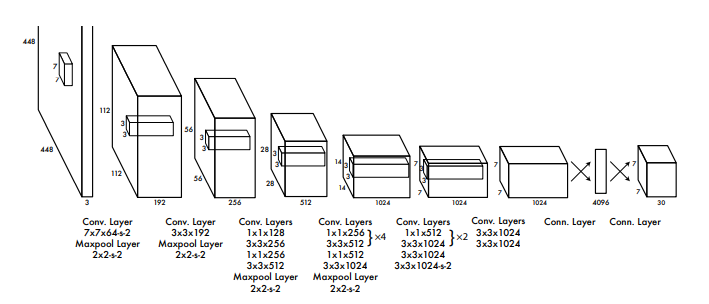
\includegraphics[scale = 0.95]{YOLOv5/yoloarchitecture.PNG}
  \caption{YOLO architecture ~\cite{redmon2016you}}
  \label{Figure 9}
\end{figure}

The input of the model is the image (pixels) and the output is the prediction (image with bounding boxes). The shape and size of the bounding boxes are pre-defined. The model will later adapt the box according to the prediction, by adding an eventual offset on the prior to match the prediction.

\bigskip

Since then, different versions of YOLO came out : YOLO ~\cite{redmon2016you}, YOLO9000 ~\cite{redmon2017yolo9000}, YOLOv3 ~\cite{redmon2018yolov3}, YOLOv4 ~\cite{bochkovskiy2020yolov4} and the latest one is YOLOv5 (May 2020 by Ultralytics) ~\cite{yolov5}, the one that will be used in this project. One of the differences with the first YOLO version is the size of bounding boxes : in the first version, we would pre define (hand pick) the sizes of the bounding boxes, however, since YOLOv2, the size of the boxes is found by running a k-means clustering. Thus we can get better priors for the model. 

\subsubsection{Finding the bounding boxes}

Let's look at how the YOLO algorithm work. First we divide the image into small cells (sub-images) and find the wanted varroa mites in each cell. Each sub-image has a pre-defined maximum number of bounding boxes.

\bigskip

Each bounding box will be defined such as : 

\begin{align}
    y &= \begin{bmatrix}
           P_c \\
           b_x \\
           b_y \\
           b_h \\
           b_w \\
           c_1 \\
           c_2 \\
           \vdots \\
           c_{n}
         \end{bmatrix}
 \end{align}
 
 \begin{enumerate}
     \item $P_c$ is the probability of a bounding box containing an object.
     \item $b_x$ and $b_y$ are the coordinates of the box (between 0 and 1 and position inside the cell).
     \item $b_h$ and $b_w$ are the width and height of the bounding box (between 0 and 1 and normalised according to the size of the cell).
     \item $c_1$, $c_2$ ... $c_n$, if there are n classes, are the Conditional Class Probability
 \end{enumerate}
  The Conditional Class Probability is the probability that an object is of a certain class given that it is a relevant object to detect (the mathematical expression would be $P(Class_i \mid Object)$). The closer to 1 the value is, the more likely that the detected object is part of that class. We should also have that the sum of all the $c_1$, $c_2$ ... $c_n$ is equal to 1. Ideally, we would want that the highest value is the closest to 1 and the others to 0. 
 
 \bigskip
 \bigskip
 
 Since we have a pre assigned number of bounding boxes for each cell, it is normal that not all the bounding boxes are used. In that case, $P_c$ is just equal to 0 and all the other parameters become irrelevant.
 
 \bigskip
 
 Thus, for each cell we get a tensor of size $B \cdot (5+C)$ with B the number of bounding boxes per cell and C the number of classes. The final tensor (all the image) will be of size $$S \cdot S \cdot (5+C) \cdot B$$ with $S \cdot S$ the number of cells in the image. 
 
\newpage

\subsubsection{IoU, Confidence score and Non max suppression}

Now let's look at how the network will find the prediction.
The first step is to compute the Intersection Over Union of the bounding box of the detected varroa with the ground truth, meaning that we will evaluate the common area and total area occupied by the bounding box and the Ground Truth (GT) (\hyperref[Figure 10]{Figure 10}).

\begin{figure}[!ht]
  \centering
  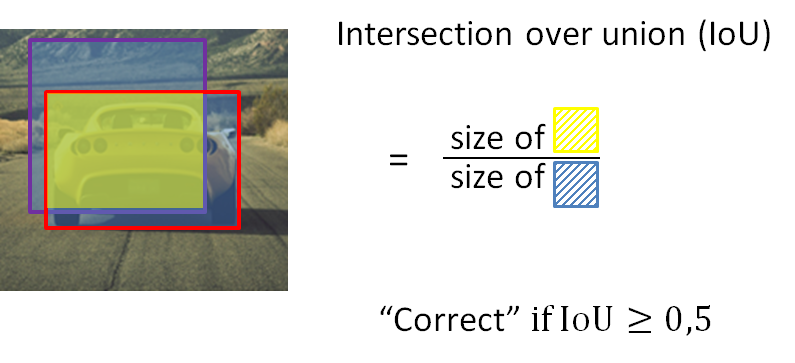
\includegraphics[scale=0.75]{metrics/IoU.png}
  \caption{Intersection over Union}
  \label{Figure 10}
\end{figure}

\bigskip

Then, the algorithm will eliminate all the boxes that have an IoU under a specific threshold (usually 0.5). Any threshold value higher could be used but would eliminate a lot of potential bounding boxes that should have been selected, but would also give a better guarantee that the predicted boxes are correct (Precision will increase but on the other hand the Recall will go down, \hyperref[Section 3.1.1]{Section 3.1.1}).

\bigskip
\bigskip

The machine will then compute the Confidence Score : $$CS = P_c \cdot IoU_{GT}$$ with $P_c$ the probability of the bounding box containing an object (varroa in our case) while $IoU_{GT}$ is the IoU between the bounding box and the ground truth.

\bigskip

Although our machine only needs to detect one class, it is worth looking at the case of a multi-class identifying network. Computing the confidence score is not enough anymore and we also need to compute the class-specific confidence score (CSCS) such as 
$$CSCS = P(Class_i \mid Object) \cdot P_c \cdot IoU_{GT} = P(Class_i) \cdot IoU_{GT}$$

\bigskip

All the boxes now have a confidence score, however the algorithm most probably detected several bounding boxes for a same varroa, and now needs to eliminate the unnecessary boxes.

\bigskip

The machine uses  non max suppression to remove the redundant bounding boxes. It will first select the box with the highest confidence as the main bounding box and the one to output. It will then compute the IoU between the box of max confidence and the rest of the boxes. If the IoU is higher than 0.5, the other box will be removed. In the \hyperref[Figure 11]{Figure 11}, the boxes to keep are the green ones and the ones to remove are the red ones as they are redundant and represent objects that were already detected. We keep the boxes with an IoU of less than 0.5 because in that case it is very likely that they do not actually bound the same detected object but rather two different varroa mites.

\begin{figure}[!ht]
  \centering
  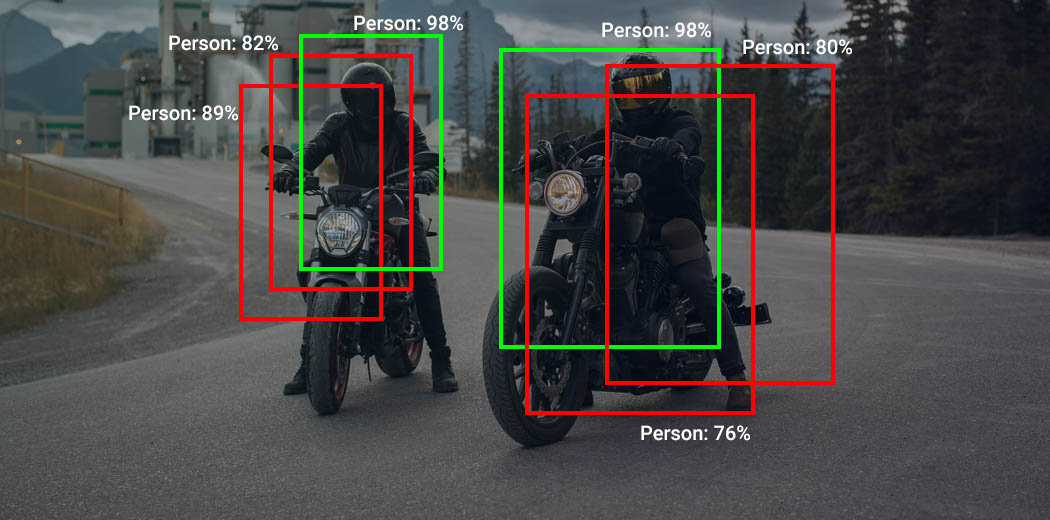
\includegraphics[scale=0.35]{metrics/nonmaxsuppression.jpg}
  \caption{Non Max suppression ~\cite{nonmax}}
  \label{Figure 11}
\end{figure}


\bigskip

\subsubsection{Network sizes}

There exists different size for the YOLOv5 model (\hyperref[Figure 12]{Figure 12}). The bigger the network, the better the results will be, but it will take more time to train. In the scope of this project, we will only focus on the YOLOv5s, which is the smallest available network. It will be the fastest one to train and we could still get good the results that are not far off the medium size network. We can see that on the \hyperref[Figure 13]{Figure 13} (below), the YOLOv5s is the fastest one to train. Although it has the worst performance, it can, in some cases, over-perform the other networks if it is trained properly.
Moreover, it is the lightest network and since we encountered several memory GPU problems, the small network would be the one with the least problems. 

\begin{figure}[!ht]
  \centering
  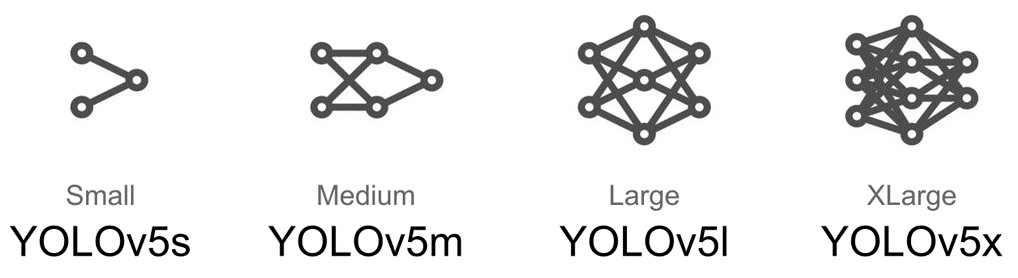
\includegraphics[scale=0.55]{YOLOv5/networksize.jpg}
  \caption{Different network sizes ~\cite{yolov5size}}
  \label{Figure 12}
\end{figure}

\begin{figure}[!ht]
  \centering
  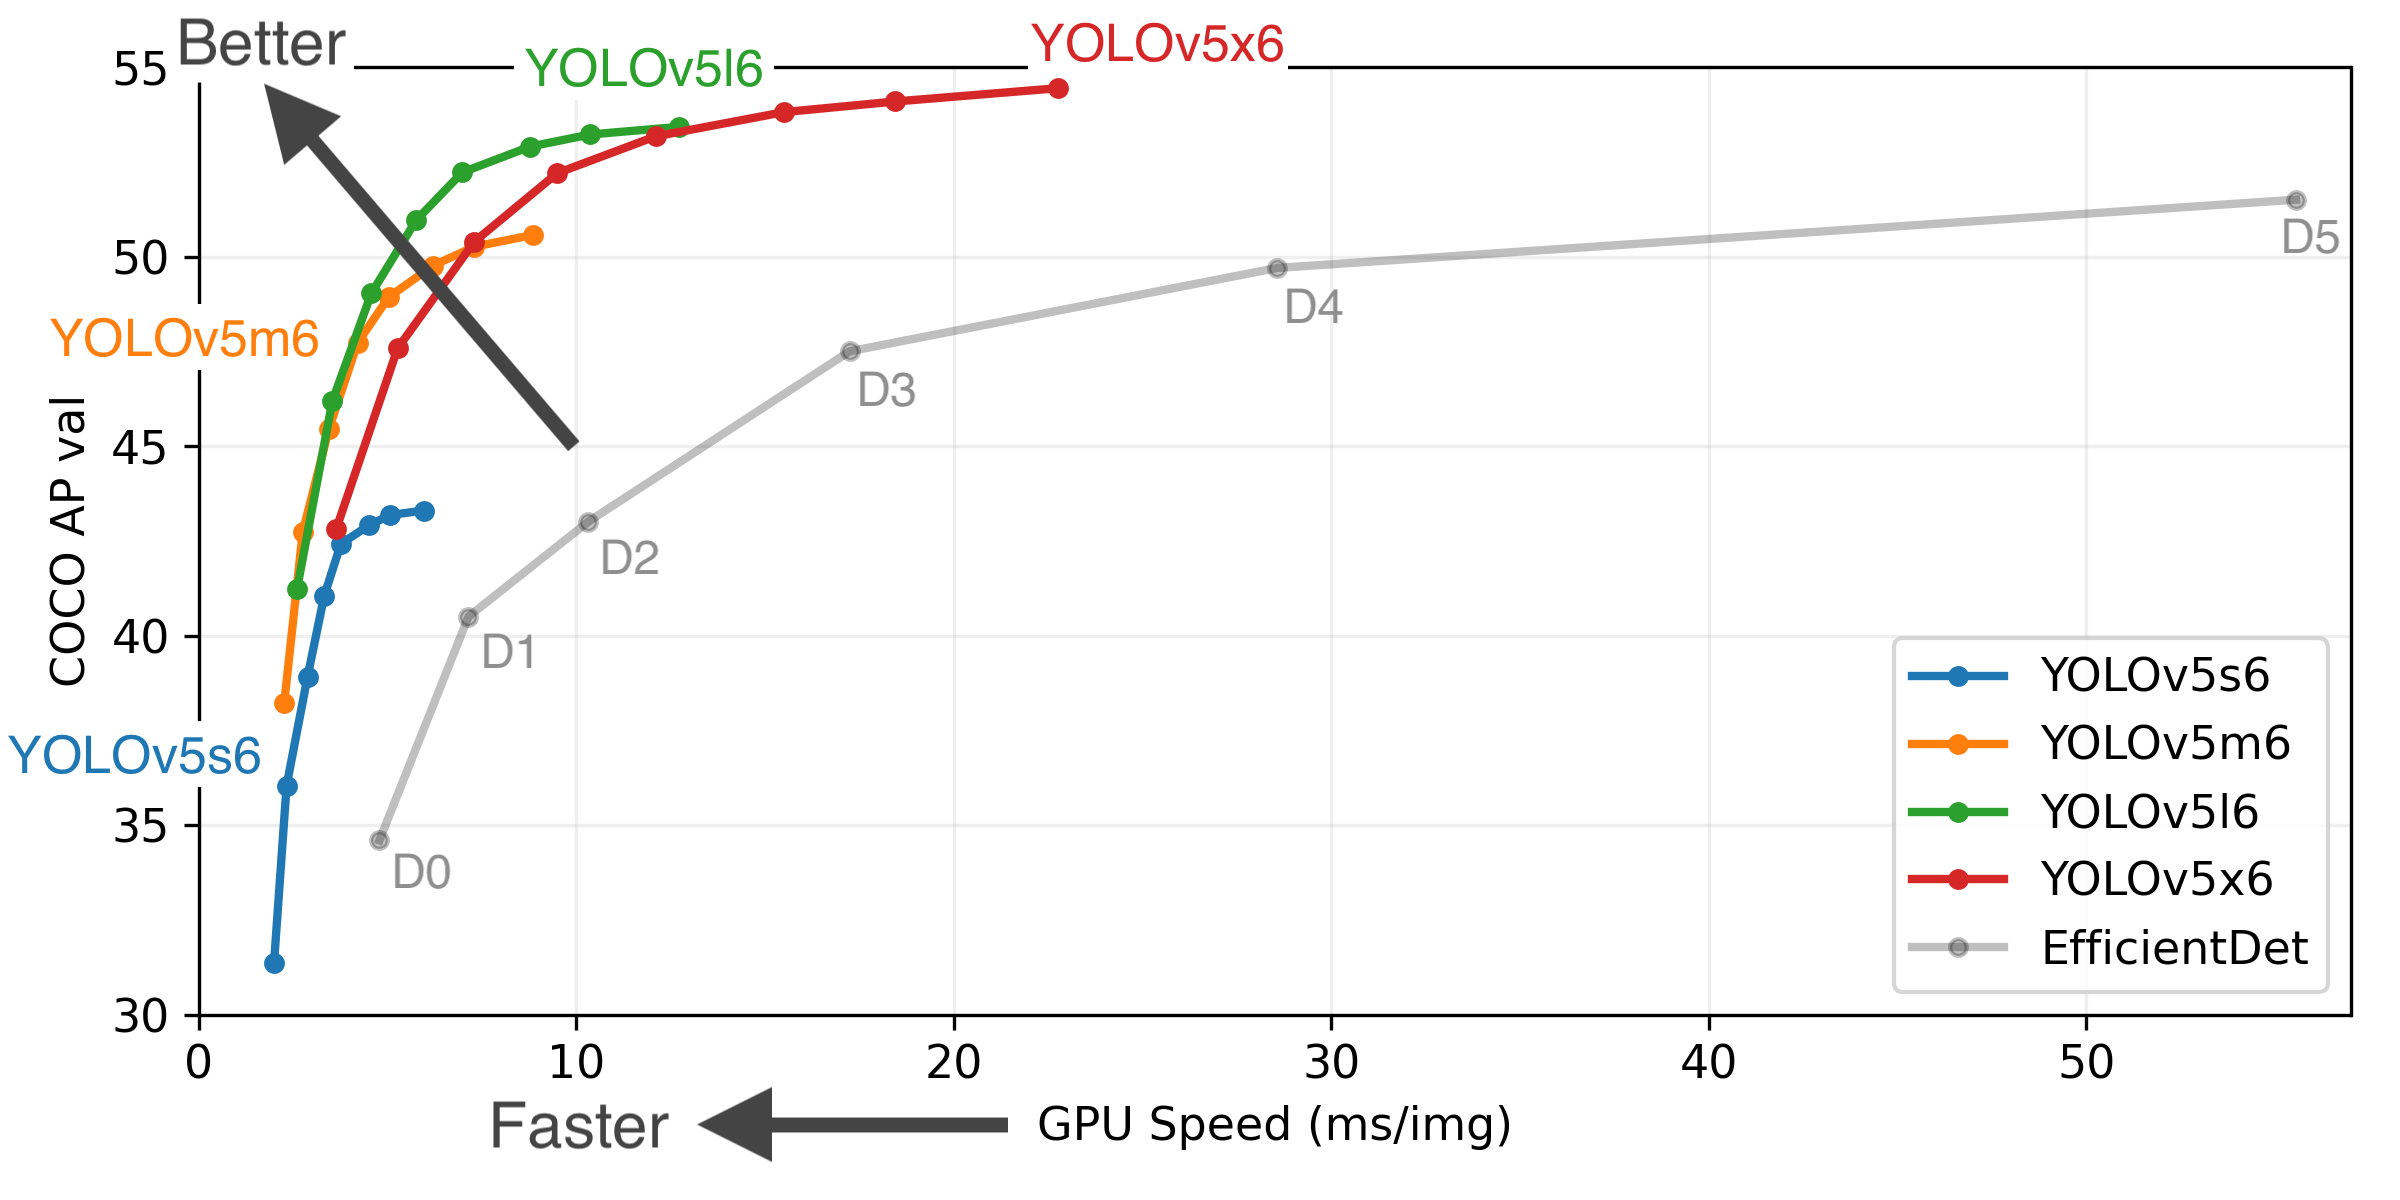
\includegraphics[scale=0.75]{YOLOv5/performance.png}
  \caption{The networks performance ~\cite{yolov5}}
  \label{Figure 13}
\end{figure}


\newpage
\section{Methods}

\subsection{Metrics}

We previously claimed that the algorithm is more efficient than a human, but how can a machine measure the efficiency and be sure that it detected a varroa inside a specific bounding box ? 



\subsubsection{Precision and Recall}
\label{Section 3.1.1}

We previously saw how does the machine determine the bounding boxes, but now it is time to look at whether the machine did a good job. A direct analysis would be to look at the number of correct guesses and bad predictions : 

\begin{itemize}
  \item True Positive (TP) : The varroa that the machine actually detected.
  \item False Positive (FP) : The object is not a varroa but the machine predicted it as a varroa.
  \item False Negative (FN) : The object is indeed a varroa but the machine did not predict it as a varroa.
  \item True Negative (TN) : The object is not a varroa and the machine did not predict it as a varroa.
\end{itemize}

We can use use these notions to do more elaborate analysis on the effectiveness of the network. Therefore we compute the following :


\begin{itemize}
  \item Precision : $P = \frac{TP}{TP + FP}$. It evaluates if the detected objects (varroa mites) were really varroa. In other words, if the machine made the correct guesses. A value of 1 would mean that all the bounding boxes actually contain a real varroa.
  \item Recall : $R = \frac{TP}{TP + FN}$. It evaluates if all the varroa mites were detected. In other words, if the machine did not forget to detect some varroa and did not leave some undetected. A value of 1 would mean that all the varroa mites on the images were detected
  \item $F1 = 2 \cdot \frac{P \cdot R}{P + R}$. It is a combination of both Precision and Recall. We want it to be the closest to 1, as it would mean that the Precision and Recall are really good.
\end{itemize}

\begin{figure}[!ht]
  \centering
  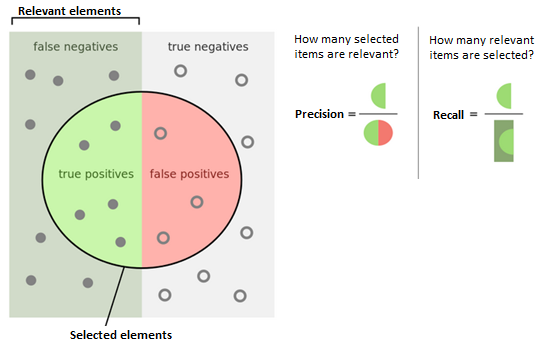
\includegraphics[scale=0.65]{metrics/precisionrecall.png}
  \caption{Precision and Recall ~\cite{precision}}
  \label{Figure 14}
\end{figure}

\bigskip

Thus, increasing the IoU threshold would increase the precision as the detected objects will more likely be varroa mites, but on the other hand, the algorithm will miss out on a lot of varroa therefore the recall will drop.

\bigskip
\bigskip

\subsubsection{AP and mAP}

Another good indicator of the efficiency is  the Average Precision AP: it is the area under the curve precision-recall. Thus, it is defined as $AP = \int_{0}^{1} p(r) dr$. The closer the value is to 1, the better it is as both the recall and precision are close to 1. Since we have different values of P and R depending on the $IoU_{GT}$ threshold, we have different values for the AP (usually the best AP would be for the IoU = 0.5). Hence it is relevant to compute the mean Average Precision : $mAP = \frac{1}{n} \sum_{i = 0.5}^{0.95} AP_i$ with n being the number of IoU threshold taken under consideration and $AP_i$ the AP for a threshold i (\hyperref[Figure 15]{Figure 15}). 

\begin{figure}[!ht]
  \centering
  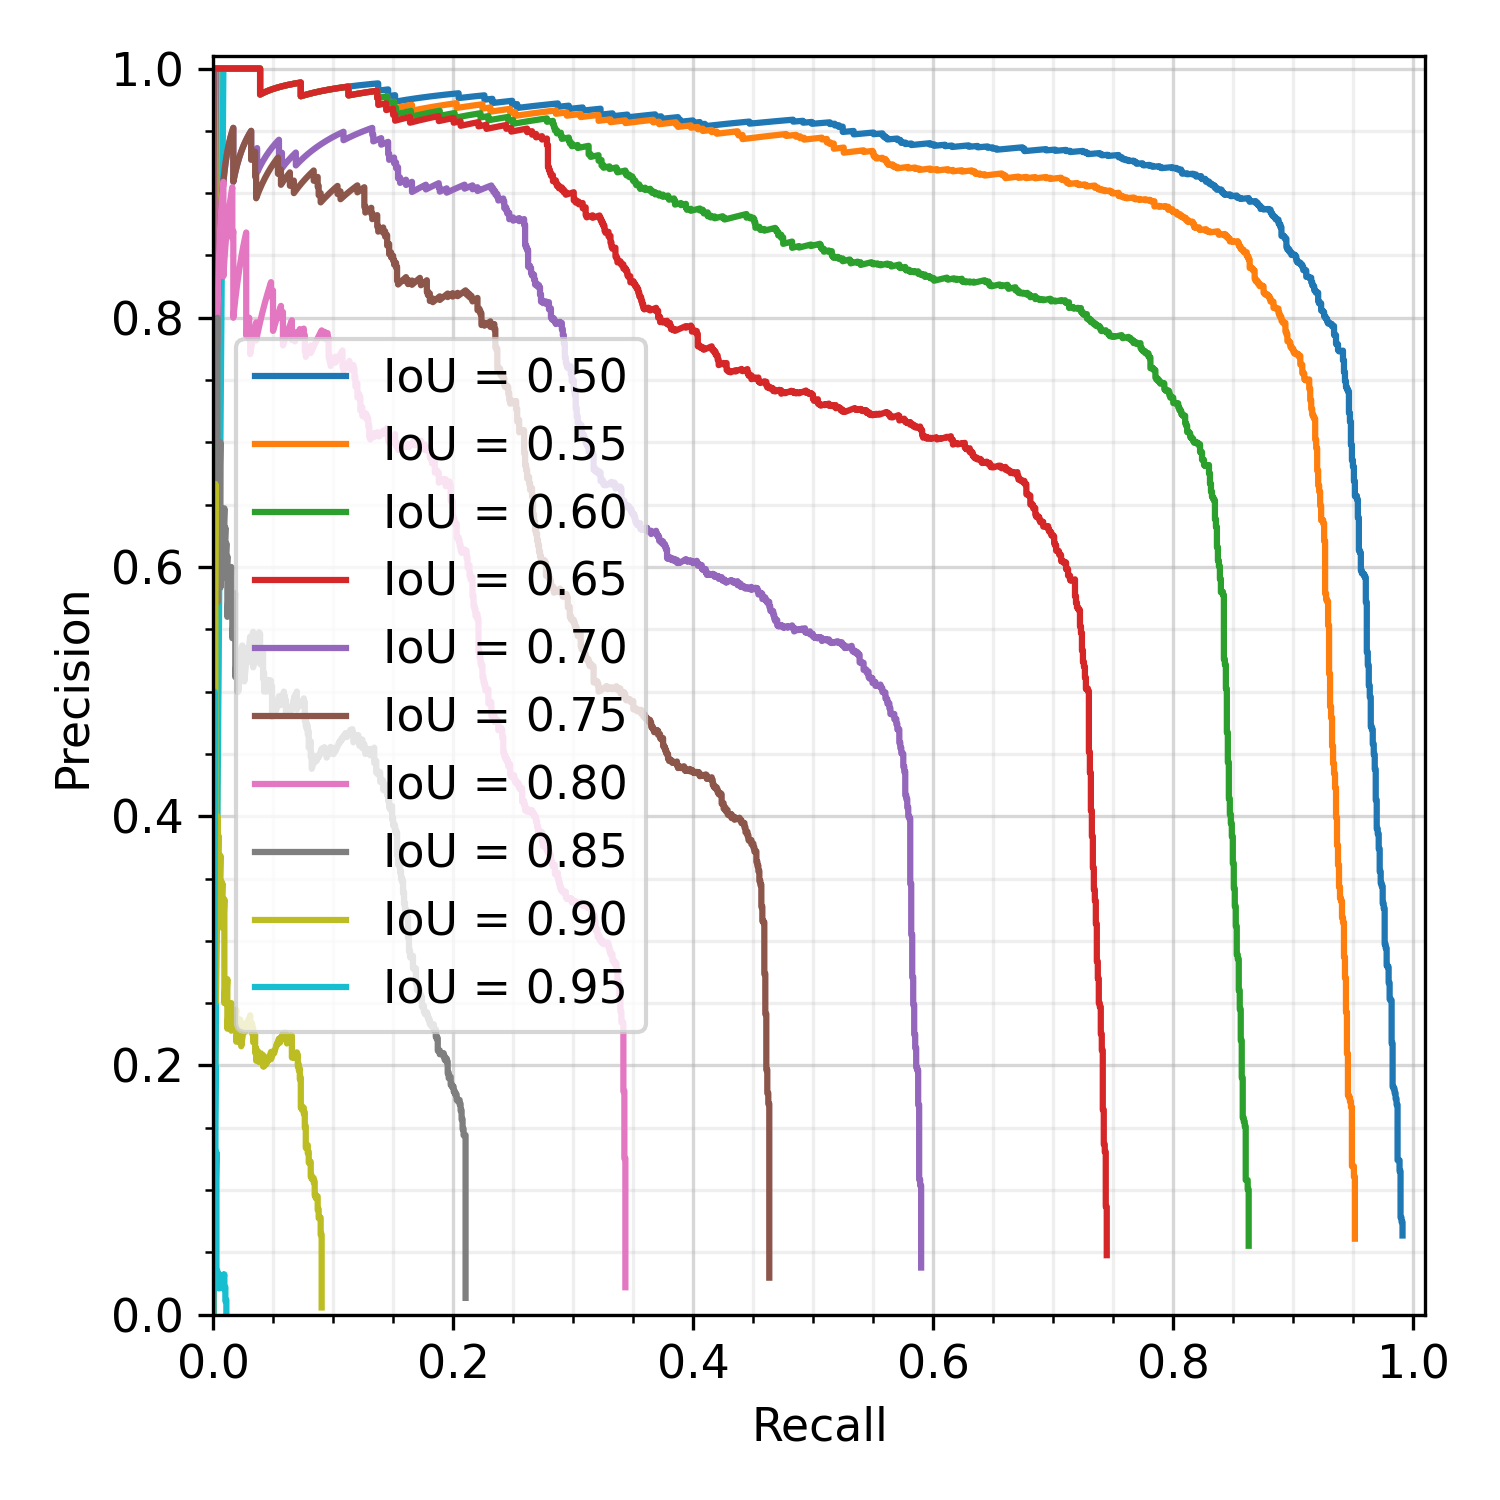
\includegraphics[scale=0.75]{metrics/mAP.png}
  \caption{Example of APs for different IoU threshold values}
  \label{Figure 15}
\end{figure}

\bigskip

Therefore, the mAP would be the average of all the areas under the curves of \hyperref[Figure 15]{Figure 15}.

\subsection{Dataset}

Our model needs to determine the resolution of the image and the mean size of the varroa mites, that depends on the position or angle of the camera. To estimate the resolution and size of the varroa,  the beekeeper places a  coin in the board which is used a reference. Once the resolution of the image is estimated, the image is classified into three categories, depending on the mean size  of the varroa mites, and then re-sampled: 

\begin{itemize}

    \item Low Resolution if the mean diameter of the varroa mites is lower than 24 pixels. After re-sampling, the mean diameter becomes 18 pixels.
    \item Mid Resolution if the mean diameter of the varroa mites is between 24 and 32 pixels. After re-sampling, the mean diameter becomes 24 pixels.
    \item High Resolution if the mean diameter of the varroa mites is higher than 32 pixels. After re-sampling, the mean diameter becomes 32 pixels.
\end{itemize}

\bigskip

It was proven in the last semester project report for ApiZoom ~\cite{stefano} that separating the images into 3 categories will increase the performance of the models, instead of using only one model for all the images. It was also found that the best network for high resolution images is the one trained with the high resolution dataset, the best network for mid resolution dataset is the network trained with the low resolution images (we just need to down-sample the mid resolution images) and lastly, the best network for the low resolution images is the one trained with the low resolution dataset.

\bigskip

In this project, only high resolution images were used: we have a total of 6633 sub-images split into 2 categories : 6411 for training part and 222 for testing. Working with only the high resolution images allowed us to have an exclusive high resolution network, that will be very efficient when fed with a high resolution image. The reason this project resolves around the high resolution images is because it is the smallest dataset and training/evolving (\hyperref[section 4]{Section 4}) is really time consuming, therefore, the smaller dataset will be faster to be done.

\bigskip

\subsubsection{Down-sampling images}

We usually have a limited number of images for each dataset, and sometimes it would be great to have more images. 
In our case, since we have 3 different datasets, we can easily increase the mid or low resolution datasets by "downgrading" high resolution images (just like we re-sampled them to have a mean varroa size of 32 pixels, we can lower the resolution to have 24 or 18). The same can be done with mid resolution to low resolution (\hyperref[Figure 16]{Figure 16}).

\begin{figure}[!ht]
  \centering
  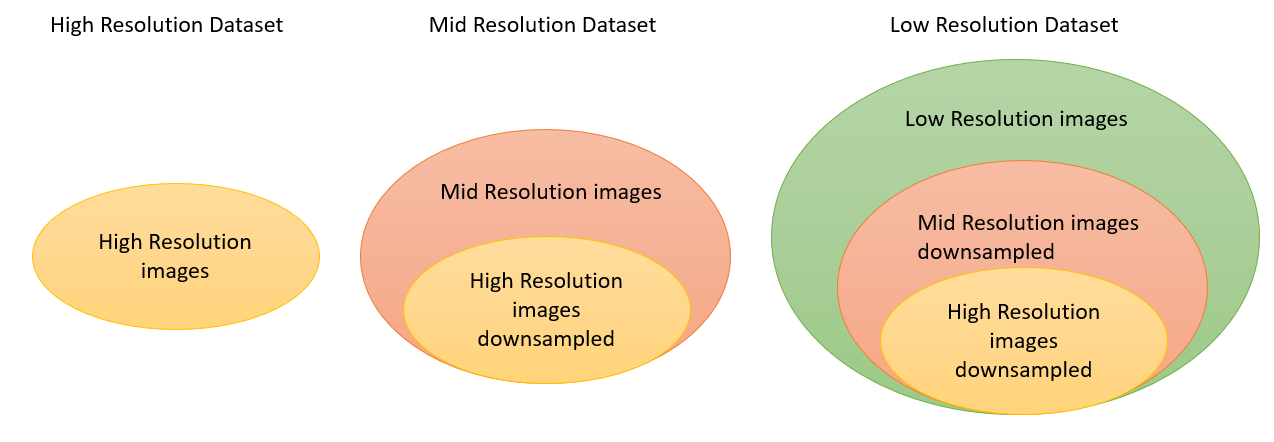
\includegraphics[scale=0.45]{dataset/datasets.PNG}
  \caption{The different datasets}
  \label{Figure 16}
\end{figure}

\bigskip

\subsubsection{Data Augmentation techniques}

Now let's look at different data augmentation techniques. They will allow us to increase our datasets without getting new images from the website: 

\bigskip

Let's first look at the Mosaic Augmentation :
We first have to resize all the images of a certain dataset to the same size (we can add some padding edges so the images are squares) and then combine 4 images together. We then proceed to extract one image which is a combination of the 4 old images and thus obtain a new image that could be fed to the network (\hyperref[Figure 17]{Figure 17}).

\begin{figure}[!ht]
  \centering
  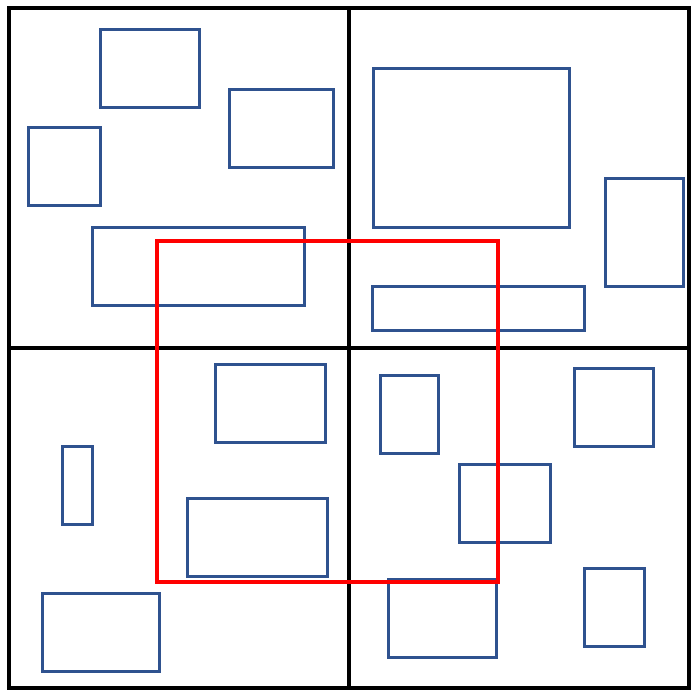
\includegraphics[scale=0.75]{dataset/mosaic.PNG}
  \caption{Example of a mosaic augmentation}
  \label{Figure 17}
\end{figure}

\newpage

Another data augmentation technique would be to rotate, or flip, or even shear the image (\hyperref[Figure 18]{Figure 18}). 

\begin{figure}[!ht]
  \centering
  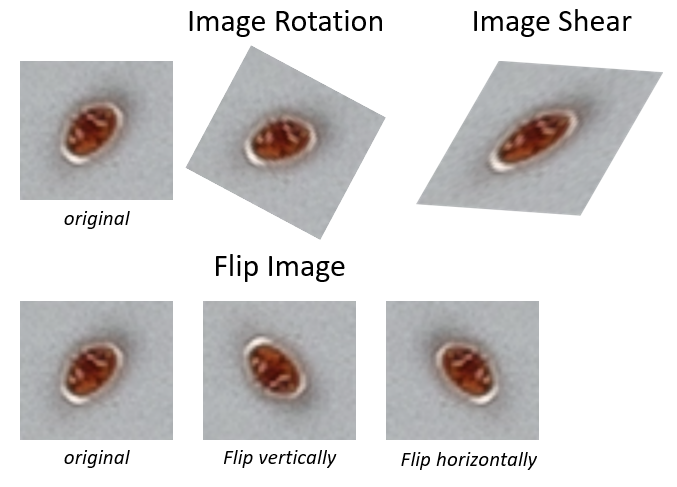
\includegraphics[scale=0.75]{dataset/augmentation.PNG}
  \caption{Image Shear, Rotation and Flip}
  \label{Figure 18}
\end{figure}

\bigskip

We can also scale or change the colour space adjustments, such as presented in the examples below (\hyperref[Figure 19]{Figure 19}):

\begin{figure}[!ht]
  \centering
  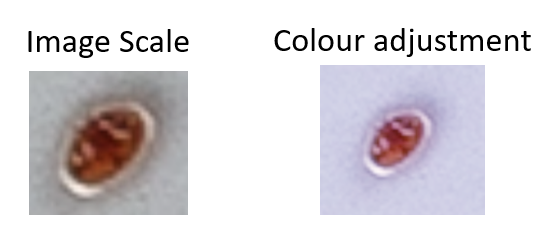
\includegraphics[scale=0.75]{dataset/scalecolour.PNG}
  \caption{Scale and colour adjustments}
  \label{Figure 19}
\end{figure}

The original image is the same as the one used for \hyperref[Figure 18]{Figure 18}

\newpage
\section{Improving the model}
\label{Section 4}

\subsection{Previous results}


The high resolution small network was previously trained last semester ~\cite{stefano} with a similar dataset for training and testing. The default hyperparameters of YOLOv5 were first used, the values of Image rotation, Image translation, Image scaling and Image shear were handpicked and changed in an attempt to optimise the network. \hyperref[Table 1]{Table 1} presents the obtained results while \hyperref[Table 2]{Table 2} indicates the 'optimised' hyperparameters values (in green are the changed values of hyperparameters).


\begin{table}[h!]
\centering
\begin{tabular}{|c|c|c|c|c|} 
 \hline
 Resolution &  Precision & Recall & F1 & Hyperparameters \\ [0.5ex] 
 \hline\hline
 High & 0.803 & 0.841 & 0.8215 & Default \\ 
 High & 0.849 & 0.854 & 0.851 & Optimised \\
 
 \hline
\end{tabular}
\caption{Training comparison}
\label{Table 1}
\end{table}

\begin{table}[h!]
\begin{center}
    \begin{tabular}{| l | l | l | l | l |}
    \hline
    lr0: 0.01 & lrf: 0.2 & momentum: 0.937 & weight\_decay: 0.0005 & warmup\_epochs: 3.0 \\
    giou: 0.05 & cls: 0.5 & cls\_pw: 1.0 & warmup\_bias\_lr: 0.1  & warmup\_momentum: 0.8 \\
    obj: 1.0 & obj\_pw: 1.0 & IoU\_t: 0.20 & anchor\_t: 4.0 & fl\_gamma: 0.0 \\
    hsv\_h: 0.015 & hsv\_s: 0.7 & hsv\_v: 0.4 & \textcolor{green}{degrees: 5.0} & \textcolor{green}{translate: 0.3} \\
    \textcolor{green}{scale: 0.8} & \textcolor{green}{shear: 5.0} & perspective: 0.0 & flipud: 0.2 & fliplr: 0.5 \\
    mosaic: 1.0 & mixup: 0.2 & & & \\
    \hline
    \end{tabular}
    \caption{Hyperparameters previously used}    
    \label{Table 2}
\end{center}
\end{table}

The 4 hyperparameters changed were deemed as the most important ones and were obtained by just guessing and trying out a few combinations. They are not the result of a specific tuning or evolution.

\bigskip

We also trained the network with the hyperparameters of \hyperref[Table 2]{Table 2} (except scale: 1.4), but with a more recent version of YOLOv5 and obtained slightly better results :

\bigskip

\begin{table}[h!]
\centering
\begin{tabular}{|c|c|c|} 
 \hline
 Parameter &  Previous report ~\cite{stefano} & Initial training's results \\ [0.5ex] 
 \hline\hline
 Precision & 0.849 & 0.888 \\ 
 Recall & 0.854 & 0.88 \\
 F1 & 0.843 & 0.884 \\

 \hline
\end{tabular}
\caption{Training comparison}
\label{Table 3}
\end{table}

\subsection{Hyperparameters}

Since we noticed a slight improvement in the results, evolving the hyperparameters would allow us to obtain the best possible results. It is a much more advanced method than just guessing random combinations of a few important hyperparameters as it will allow us to find the best hyperparameters for a specific network. We first have to define the fitness function as a weighted combination of metrics: AP at IoU = 0.5 contributes 10\% of the weight and mAP@0.5:0.95 contributes the remaining 90\%. The evolution will run for several hundreds of generations (at least 300), with each generation being 10 epochs. At each generation, it will run a different scenario with different hyperparameters values (between a specific range : \hyperref[Table 4]{Table 4}) and find the one that maximises the fitness.

\bigskip
 
\begin{table}[h!]
\centering
\begin{tabular}{|c|c|c|c|} 
 \hline
 Hyperparameter &  Mutation scale & Lower limit & Higher limit \\ [0.5ex] 
 \hline\hline
 lr0 & 1& 1e-5& 1e-1  \\ 
 lrf& 1& 0.01& 1.0 \\ 
 momentum & 0.3& 0.6& 0.98 \\ 
 weight\_decay &1& 0.0& 0.001 \\ 
 warmup\_epochs &1& 0.0& 5.0 \\ 
 warmup\_momentum & 1& 0.0& 0.95 \\ 
 warmup\_bias\_lr & 1& 0.0& 0.2 \\ 
 box & 1& 0.02& 0.2 \\ 
 cls & 1& 0.2& 4.0 \\ 
 cls\_pw & 1& 0.5& 2.0 \\ 
 obj&1& 0.2& 4.0 \\ 
 obj\_pw&1& 0.5& 2.0 \\ 
 IoU\_t&0& 0.1& 0.7 \\ 
 anchor\_t&1& 2.0& 8.0 \\ 
 fl\_gamma&0& 0.0& 2.0 \\ 
 hsv\_h&1& 0.0& 0.1 \\ 
 hsv\_s&1& 0.0& 0.9 \\ 
 hsv\_v&1& 0.0& 0.9 \\ 
 degrees&1& 0.0& 45.0 \\ 
 translate&1& 0.0& 0.9 \\ 
 scale&1& 0.0& 0.9 \\ 
 shear&1& 0.0& 10.0 \\ 
 perspective&0& 0.0& 0.001 \\ 
 flipud&1& 0.0& 1.0 \\ 
 fliplr&0& 0.0& 1.0 \\
 mosaic&1& 0.0& 1.0 \\ 
 mixup&1& 0.0& 1.0 \\ [1ex] 
 \hline
\end{tabular}
\caption{Hyperparameters range}
\label{Table 4}
\end{table}

\subsection{Evolution results}

After evolving for 350 generations, we get the following results (\hyperref[Figure 20]{Figure 20}). Although the new results (\hyperref[Table 5]{Table 5}) are better than the previous report's ~\cite{stefano} results, they are still underwhelming and disappointing as they are quite similar to the results obtained initially by training the network without evolving the hyperparameters.

\bigskip

Therefore, the evolution was resumed to reach a total of 500 generations (\hyperref[Figure 21]{Figure 21}). Unfortunately, the results are very similar to the 350 generations evolution, and did not really improve the situation. The evolved values of the hyperparameters can be found on the following 2 output pictures :

\begin{figure}[!ht]
  \centering
  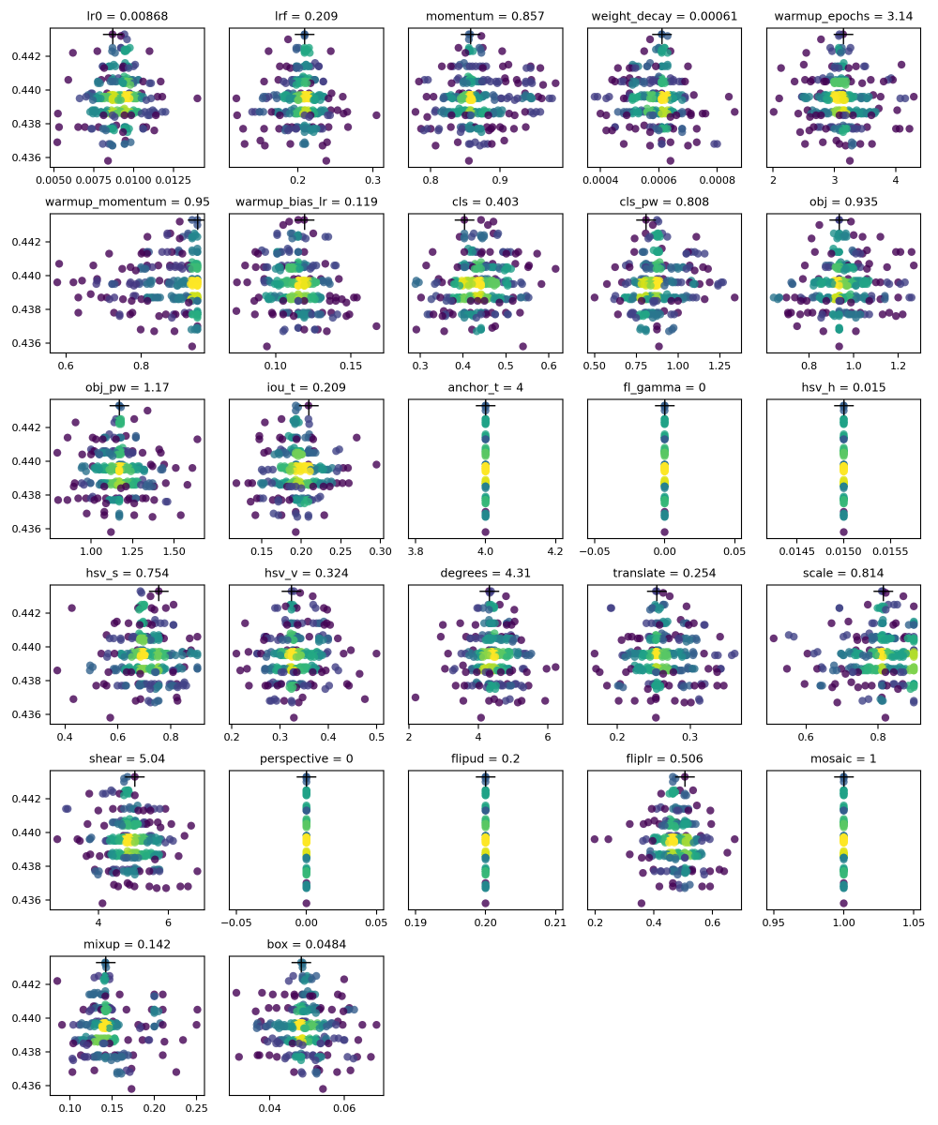
\includegraphics[scale=0.9]{evolution/evol1.png}
  \caption{First evolution results}
  \label{Figure 20}
\end{figure}

\newpage

\begin{figure}[!ht]
  \centering
  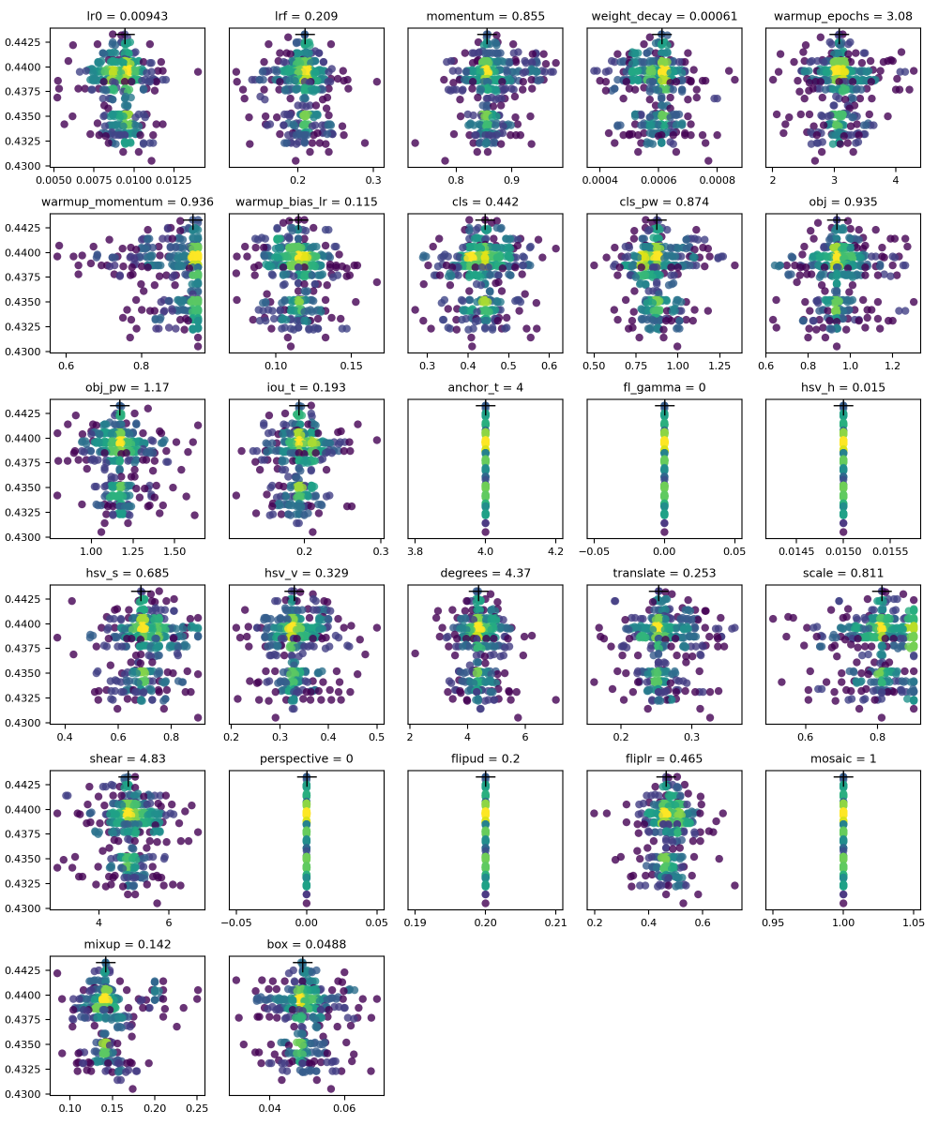
\includegraphics[scale=0.9]{evolution/evol2.png}
  \caption{Second evolution results}
  \label{Figure 21}
\end{figure}

\newpage

\begin{table}[h!]
\centering
\begin{tabular}{|c|c|c|c|c|} 
 \hline
 Parameter &  Previous report ~\cite{stefano} & Initial training's results & First evolution & Second evolution \\ [0.5ex] 
 \hline\hline
 Precision & 0.849 & 0.888 & 0.859 & 0.855 \\ 
 Recall & 0.854 & 0.88& 0.896& 0.902 \\
 F1 & 0.843 & 0.884 & 0.877 & 0.878 \\
 AP for IoU = 0.5 & N/A & 0.918 & 0.908 & 0.913 \\
 mAP & N/A & 0.426 & 0.441 & 0.421 \\ [1ex] 
 \hline
\end{tabular}
\caption{Training comparison}
\label{Table 5}
\end{table}

\bigskip

In the table, we can see the networks' performances : in the first column, we have the last report's results for a small YOLO network that with the special hyperparameters values. In the second column, we can see the results of a training that was done before the evolution with nearly the same parameters used as in the first column. Finally on the last two columns, we can see the results of the two evolutions (350 and 500 generations respectively). We can easily see that there is no improvement compared to the training done before the evolutions and therefore it is a bit disappointing.

\bigskip

We then attempted to resume the evolution for a total of 600 generations, but unfortunately, got exactly the results (hyperparameters values) as the first evolution. 

\subsection{Evolution of a few hyperparameters}

Since the evolution results were quite disappointing, we decided to redo the evolution, but this time, evolve only the most important hyperparameters : Image rotation, Image translation, Image scaling and Image shear, with all the other hyperparameters being the same as the ones from the first evolution. We get the following hyperparameters were evolved after 450 generations (\hyperref[Table 6]{Table 6}). The plot of the hyperparameters are available on the \hyperref[Figure 22]{Figure 22}.

\begin{table}[h!]
\begin{center}
    \begin{tabular}{| l | l | l | l | l |}
    \hline
    lr0: 0.00868 & lrf: 0.209 & momentum: 0.857 & weight\_decay: 0.00061 & warmup\_epochs: 3.14 \\
    giou: 0.0488 & cls: 0.442 & cls\_pw: 0.874 & warmup\_bias\_lr: 0.119  & warmup\_momentum: 0.95 \\
    obj: 0.935 & obj\_pw: 1.17 & IoU\_t: 0.193 & anchor\_t: 4.0 & fl\_gamma: 0.0 \\
    hsv\_h: 0.015 & hsv\_s: 0.685 & hsv\_v: 0.329 & \textcolor{green}{degrees: 5.53} & \textcolor{green}{translate: 0.169} \\
    \textcolor{green}{scale: 0.568} & \textcolor{green}{shear: 3.9} & perspective: 0.0 & flipud: 0.2 & fliplr: 0.465 \\
    mosaic: 1.0 & mixup: 0.142 & & & \\
    \hline
    \end{tabular}
    \caption{Hyperparameters after evolution}    
    \label{Table 6}
\end{center}
\end{table}

\newpage

\begin{figure}[!ht]
  \centering
  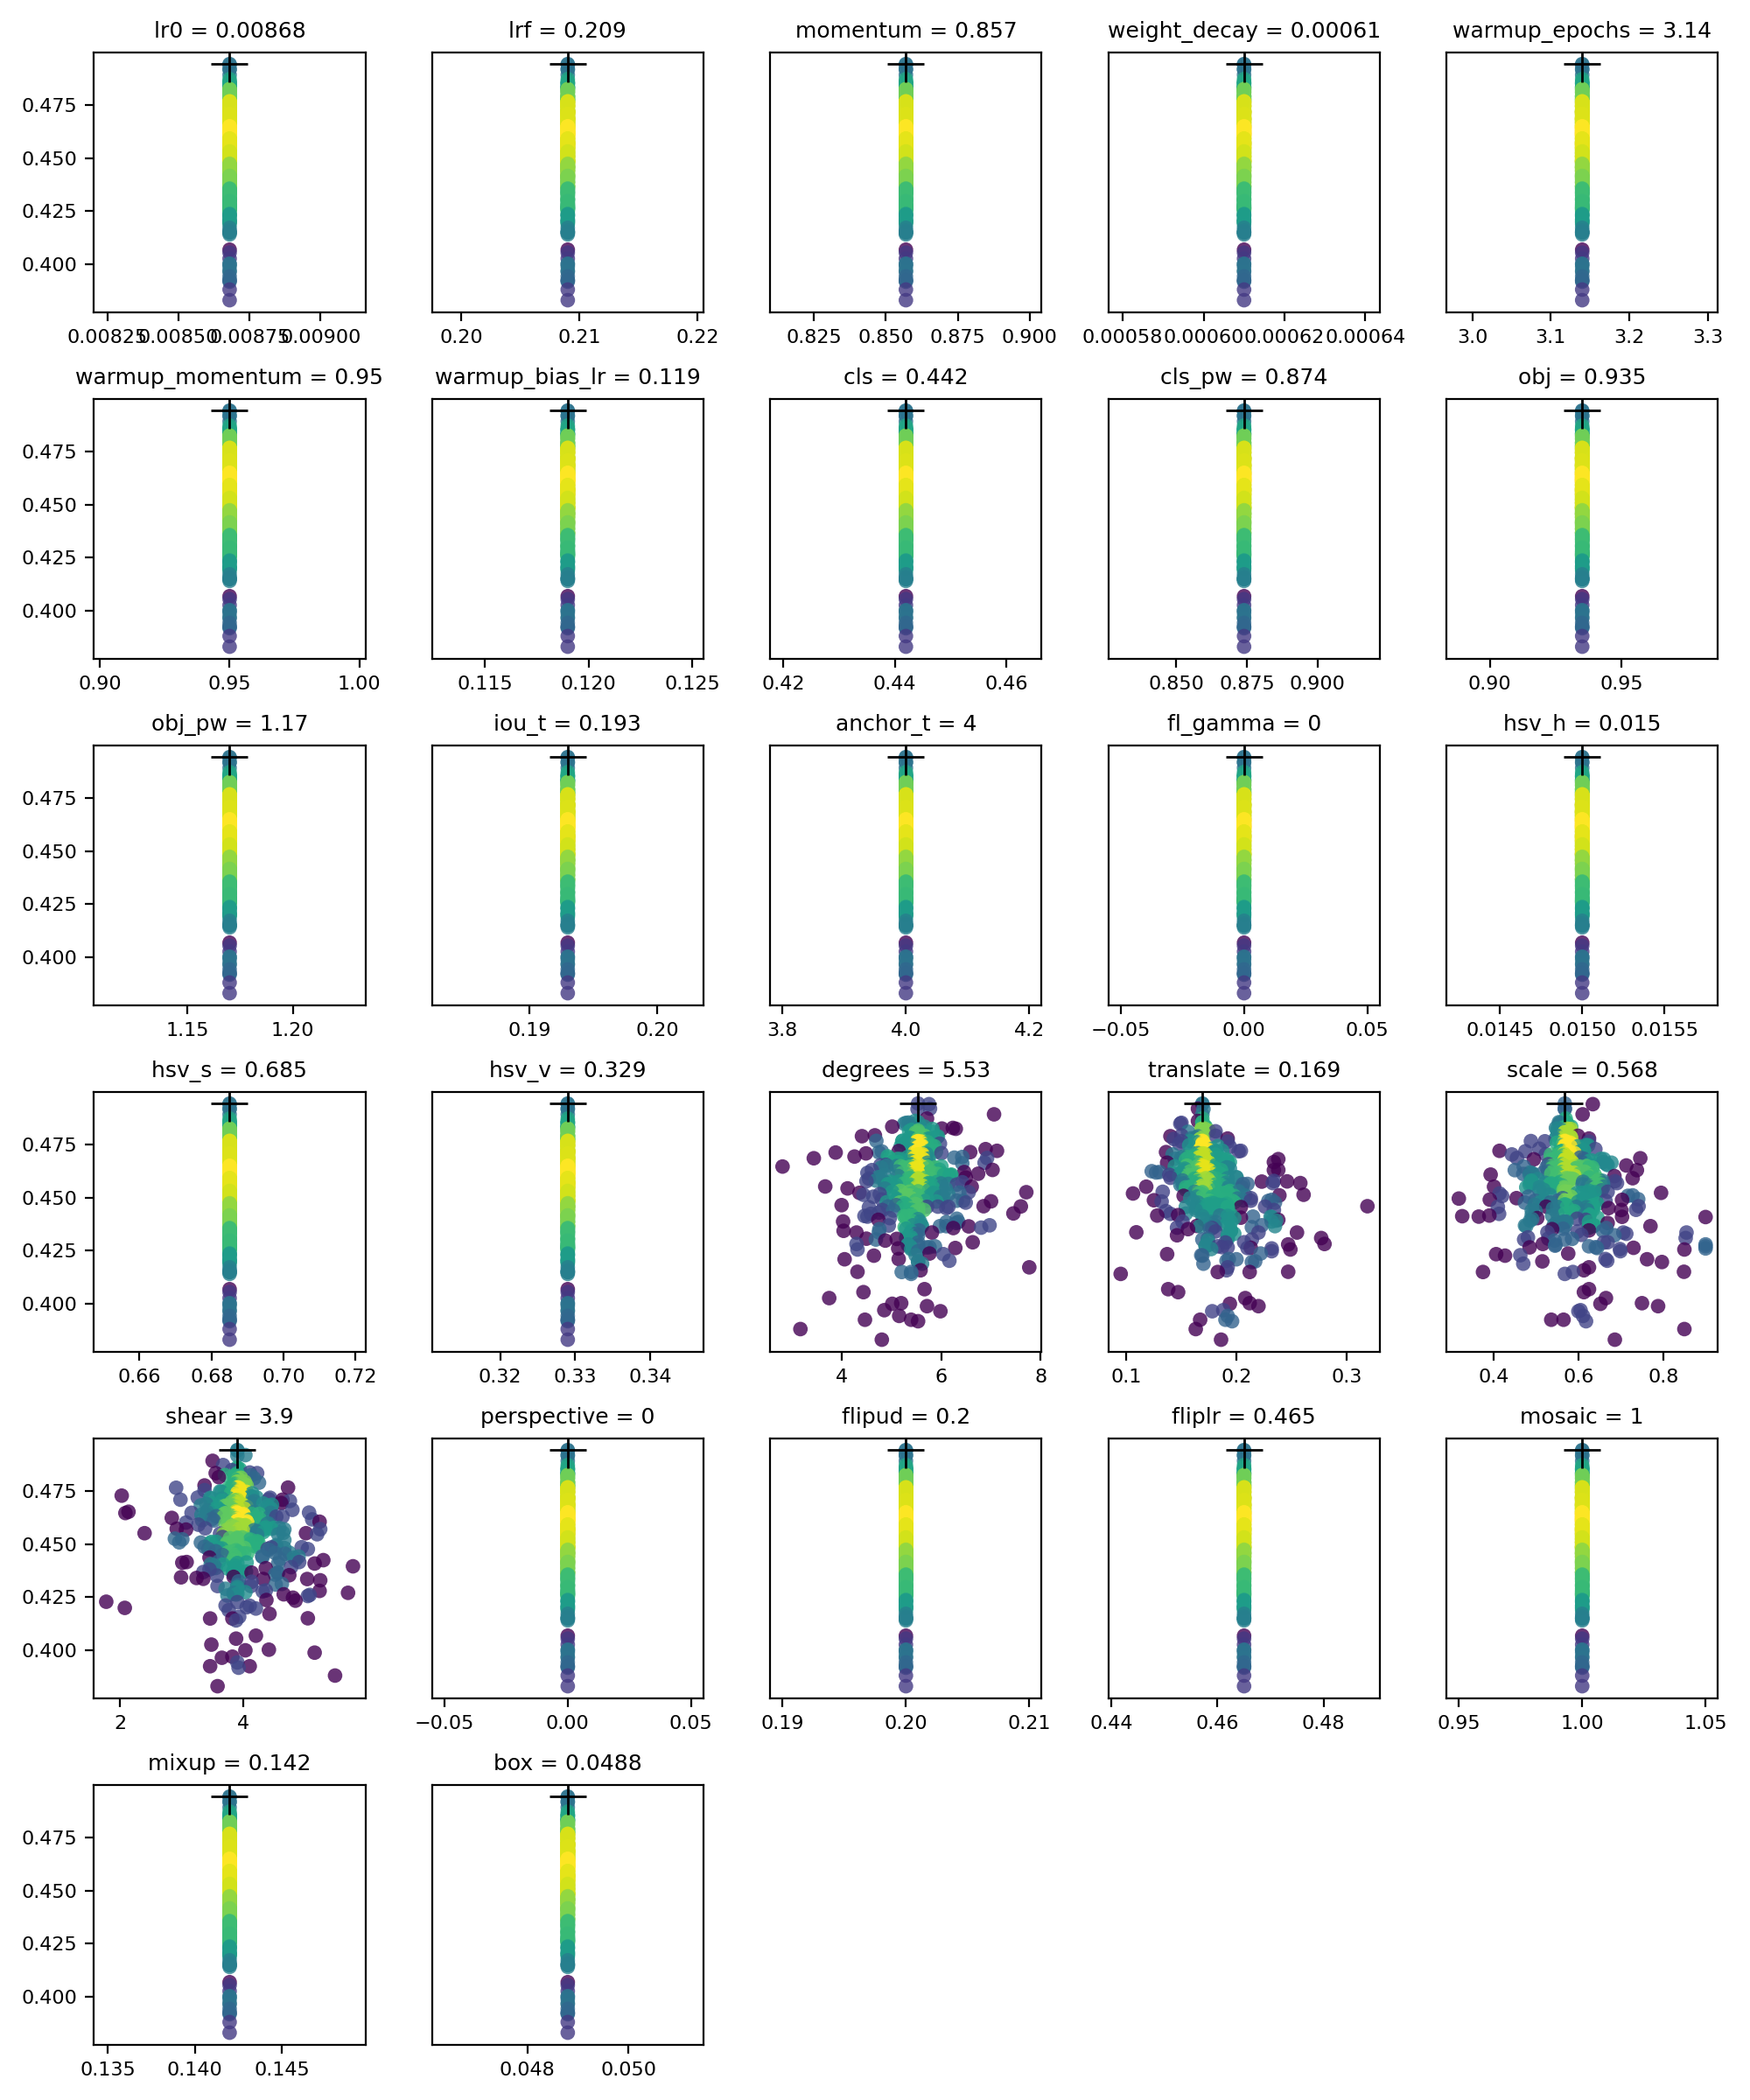
\includegraphics[scale=0.6]{evolution/evolve.png}
  \caption{Third evolution results}
  \label{Figure 22}
\end{figure}

\newpage

After testing the new hyperparameters, we get the following results :

\begin{table}[h!]
\centering
\begin{tabular}{|c|c|c|c|c|} 
 \hline
 Parameter & Initial training's results & First evolution & Second evolution & Third evolution\\ [0.5ex] 
 \hline\hline
 Precision & \textcolor{green}{0.888} & 0.859 & 0.855 & 0.877 \\ 
 Recall & 0.88& 0.896& 0.902 & \textcolor{green}{0.907} \\
 F1 & 0.884 & 0.877 & 0.878 & \textcolor{green}{0.892} \\
 AP for IoU = 0.5 & 0.918 & 0.908 & 0.913 & \textcolor{green}{0.928} \\
 mAP & 0.426 & 0.441 & 0.421 & \textcolor{green}{0.465} \\ [1ex] 
 \hline
\end{tabular}
\caption{Training comparison}
\label{Table 7}
\end{table}

\bigskip

We finally notice an improvement in the F1, AP at IoU = 0.5 and mAP at the third evolution's results. Although we are pleased that the optimised hyperparameters gave us better results compared to the previous ones, we notice that they are still in the same range as the previous ones and that the improvement is very slight.

\bigskip

\subsection{Summary of the evolution}


We tried to evolve the hyperparameters at first for 350 generations. Since we did not obtain improving results, we resumed it for another 150 generations (total of 500) and then another 100 generations (total of 600. Regrettably the network was not improved by those hyperparameters evolution.

\bigskip

At last, we tried to evolve just a few important hyperparameters for 450 generations. The new results were slightly better but still comparable to the previous ones.

\bigskip

We also notice some changes on the evolution plots (\hyperref[Figure 20]{Figure 20}, \hyperref[Figure 21]{Figure 21} and \hyperref[Figure 22]{Figure 22}). Indeed, we notice that in the \hyperref[Figure 22]{Figure 22} (evolution of just a few hyperparameters), the model was actually converging towards the optimal hyperparameters values (yellow indicates a large number of generations around that value and blue is the opposite). Meanwhile, in the \hyperref[Figure 20]{Figure 20} and \hyperref[Figure 21]{Figure 21}, we notice that the yellow area is not near the optimal hyperparameters (although for the second evolution it is nearer), meaning that the evolution might have been aborted too early, therefore being a possible explanation for why the results were unsatisfying.

\bigskip

We faced several problems throughout the evolutions : Unfortunately, each evolution was very time consuming and we were constantly facing a GPU problem that would massively slow down the training, even though we worked with a batch size of 2.

\newpage
\section{Apizoom Website}

\subsection{Uploading an image as an admin}

The first thing the user needs to do is to upload an image to the website, he then needs to choose the algorithm (YOLOv5 in our case) and lastly choose the scale: which coin he placed on the board.

Once that step is done, the machine will detect the coin on the image and draw a green circle around it to indicate that it actually found the coin (\hyperref[Figure 23]{Figure 23}). Since the algorithm is aware of the coin's diameter, it will give itself a good scale indicator and what varroa size should it expects (in pixels). 

\begin{figure}[!ht]
  \centering
  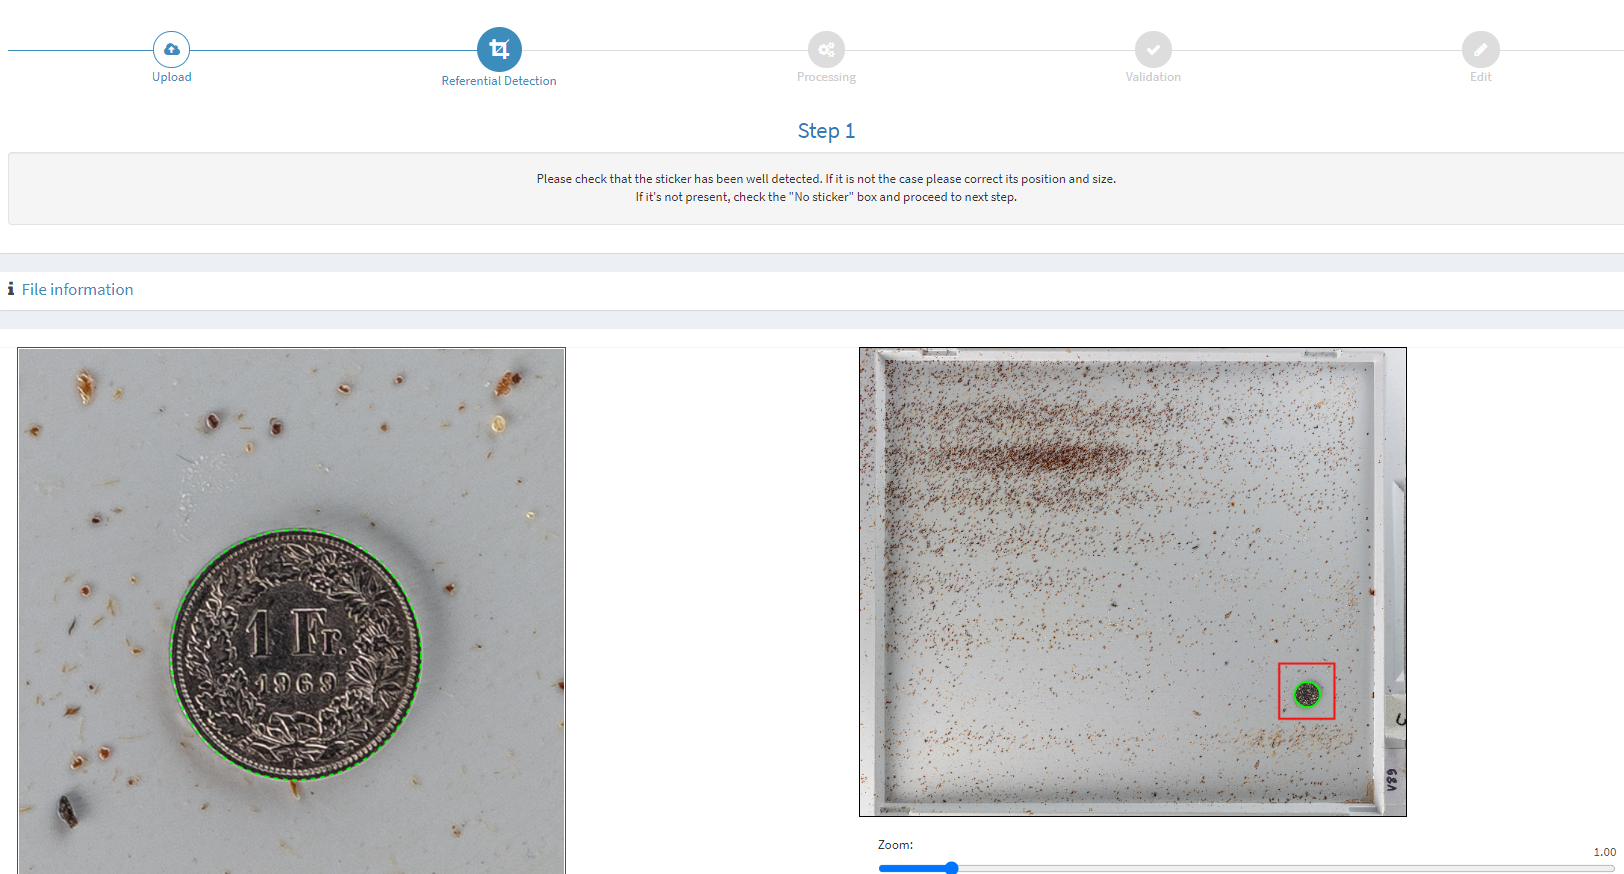
\includegraphics[scale=0.4]{website/scale.PNG}
  \caption{Coin detecting}
  \label{Figure 23}
\end{figure}

\bigskip

The machine will then divide the image into sub-images and detect the parasites on each sub-image and lastly output the full image with all the predictions and bounding boxes + confidence score. It is worth noting that it will also indicate the estimated varroa size in pixels. It is now the user's responsibility to validate each prediction ("validation" step) : he can either confirm that the machine was correct, in that case the box becomes green (true positive), or that the machine was incorrect with the box becoming red (it is not a varroa inside the box : false positive), or that he is unsure about the prediction (orange box). In the next step ("edit"), the user can add some boxes for varroa mites that the algorithm missed out on (false negative) with a blue box.

\subsection{Database}

The database used is stored with Mongo DB. We can find all the characteristics of the image : file name, selected coin ... We can also look at the array of points : all the bounding boxes on the image (TP, FP and FN). For each box, we can see the position of its top left corner, confidence score and size (width and height). These information are very important as they will allow us to recreate the image and not lose all the data once we refresh the page.

\bigskip

Mongo DB is not just useful for storing and displaying boxes from the website. It is also used as an easy way to collect more images that could be used for a future training. In that way, we can improve our dataset with picture submitted from anyone.

\subsection{Limitations of the current website}

The current website does not offer much features for manually editing the predictions done by the algorithm.

\subsubsection{Editing the boxes}

The website does not give the admin as much freedoms as he would need. The admin cannot move TP boxes (in order to adjust them). Indeed, not all the predictions are perfect and it is quite easy to notice that (\hyperref[Figure 24]{Figure 24}): 

\begin{figure}[!ht]
  \centering
  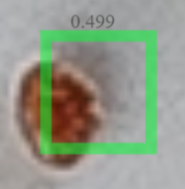
\includegraphics[scale=0.9]{limitation/misplaced.PNG}
  \caption{Bad bounding box placement}
  \label{Figure 24}
\end{figure}

Another major limitation is that the user cannot change the size of a box. Indeed, some boxes are too large or too small (\hyperref[Figure 25]{Figure 25})

\begin{figure}[!ht]
  \centering
  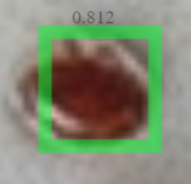
\includegraphics[scale=0.9]{limitation/small.PNG}
  \caption{Too small box}
  \label{Figure 25}
\end{figure}

We can clearly see that the bounding box for that varroa is too small and a bigger one would have been much better (\hyperref[Figure 25]{Figure 25}).

\bigskip

This step is crucial as the submitted images will be added to the dataset. It is important to have the correct position and size for the bounding boxes in our dataset.

\subsubsection{Display bugs}

The website also had a few bugs regarding the display of boxes : When created, a FN blue box would appear as a circle and when the page was refreshed, the website would show a squared box, but with an offset, making the position of the box quite inaccurate : 

 
\begin{figure}[!ht]
    \centering
    \begin{minipage}{0.25\textwidth}
        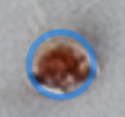
\includegraphics[width=\textwidth]{limitation/circle.PNG}
        \caption{Circle bounding box before refresh}
        \label{Figure 26}
    \end{minipage}
    \begin{minipage}{0.25\textwidth}
        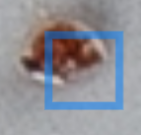
\includegraphics[width=\textwidth]{limitation/refresh.PNG}
        \caption{Bounding box after refresh}
        \label{Figure 27}
    \end{minipage}

\end{figure}

We would also notice a similar display bug when the coordinate of a box was changed : if the user would manually change the position of a bounding box (by dragging the box with the mouse \hyperref[Section 5.4.1]{Section 5.4.1}), and then refresh the page, a similar display offset would appear as the box will be slightly shifted (\hyperref[Figure 28]{Figure 28}) : 

\begin{figure}[!ht]
  \centering
  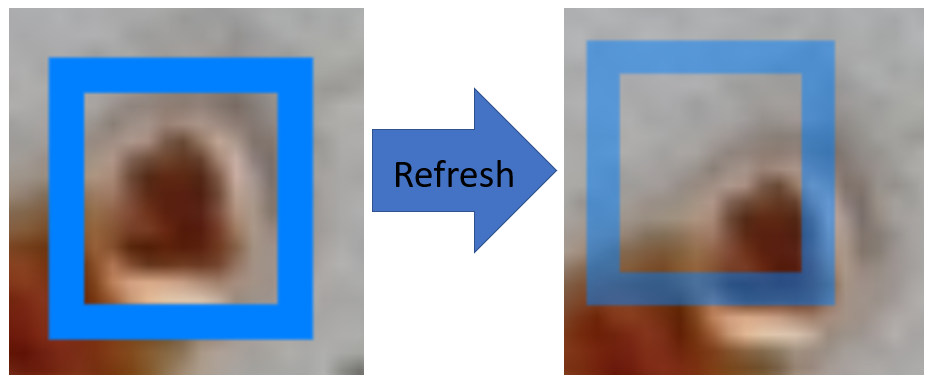
\includegraphics[scale=0.8]{limitation/offset.PNG}
  \caption{Position offset}
  \label{Figure 28}
\end{figure}


\subsection{New features}
In this section, the new features added to improve the accuracy of the bounding boxes are detailed.
These new features appear on the last step ("edit"). In addition, the way the display bugs have been solved is also presented.


\subsubsection{Editing the boxes}
\label{Section 5.4.1}

The user can now change the position of a box on the image (the position of a prediction is considered to be the top left corner of the box). He can also change its width and height. Let's look back at the previous examples, first we have the badly positioned boxes (\hyperref[Figure 24]{Figure 24}). Now we can see that the user managed to move the boxes by just dragging the new box with the mouse:

\begin{figure}[!ht]
  \centering
  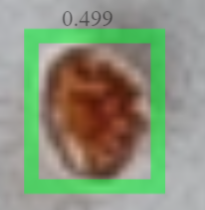
\includegraphics[scale=0.9]{features/coordinates.PNG}
  \caption{Good bounding box placement}
  \label{Figure 28}
\end{figure}

\bigskip

The user can also change the size of the box. Again, let's look back at the previous example (\hyperref[Figure 25]{Figure 25}):

\begin{figure}[!ht]
  \centering
  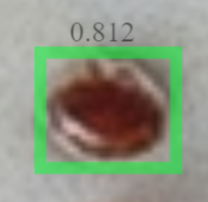
\includegraphics[scale=0.9]{features/size.PNG}
  \caption{Good size box}
  \label{Figure 30}
\end{figure}

This was made possible with the introduction of new buttons that allow the user to increase or decrease the width or height of the box (W is for width and H is for height) :

\begin{figure}[!ht]
  \centering
  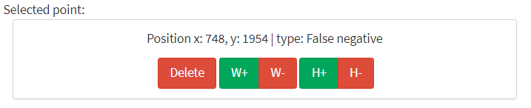
\includegraphics[scale=0.9]{features/buttons.png}
  \caption{Size controlling buttons}
  \label{Figure 31}
\end{figure}


\bigskip
\bigskip

It is also worth mentioning that any change made on the website will directly be updated on the Mongo database.


\subsubsection{Fixing the display bugs}

Both display bugs are now solved. They were caused by a "review\_offset" between the display on the screen and the coordinates on the database. It needed to be taken under consideration when changing the coordinates and updating the database. This issue is now solved and the boxes do not move when updating the image. Moreover, the FN are generated as squared boxes and not circles (we can also refresh the without any problem). An example is presented in the \hyperref[Figure 32]{Figure 32}. Once we refresh the page, the position of the bounding box does not change.

\begin{figure}[!ht]
  \centering
  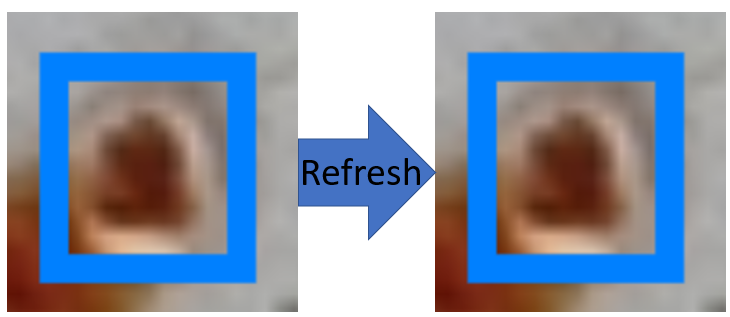
\includegraphics[scale=0.9]{features/nomove.PNG}
  \caption{Bounding Box stays in the same position}
  \label{Figure 32}
\end{figure}

\newpage

\section{Conclusion}

The project had 2 specific goals : 
\begin{enumerate}
    \item Improve the Deep Learning network by finding optimal hyperparameters.
    \item Improve the collection of new annotated images from the website by allowing the admin user to adjust inaccurate bounding boxes.
\end{enumerate}

\bigskip

For the Deep Learning part, the results were at first quite disappointing as the evolutions turned out to be very time consuming and initially did not improve the network. However, we managed to find a way to obtain some slight improvement by evolving just a few important hyperparameters.

\bigskip

Thankfully, improving the website was much more successful.  This part is really important as it would allow us to obtain better annotations and more accurate bounding boxes.  These images will then be used to enlarge the datasets for future training, therefore it is really important to have the best possible annotations. 

\bigskip

This project was my first deep learning and computer vision experience. Even though I did not get the expected results, I've learned a lot throughout the semester, whether it is on the deep learning and YOLO theory (how does the machine recognise the wanted patterns on the image) or on practice (how to train a network, how to interpret the data, how to use pytorch, how to code in javascript for the website...). Moreover, it really encouraged me to pursue my Master's degree in this field.

\bigskip

There are a lot of improvements that could be done in the future. Here are a few suggestions for the Deep Learning part :
\begin{enumerate}
    \item Evolve for a higher number of generations.
    \item Evolve the hyperparameters for the different datasets (low/mid resolution).
    \item Evolve the hyperparameters for a different network size (YOLOv5m).
    \item Try new data augmentation techniques like Image Occlusion.
    \item Evolve the network with cross validation dataset instead of using the same dataset for testing and validation.
\end{enumerate}

We can also add the new features implemented on the website to the ApiZoom application.


\bigskip

Lastly, I would like to thank my supervisor Roser Vinals Terres for constantly helping me throughout the project and always answering my questions.
I would also like to thank my supervisors Roser Vinals Terres and Prof. Jean-Philippe Thiran for giving me the opportunity to work on that amazing project. 


\newpage
\bibliographystyle{plain}
\bibliography{bibliography.bib}

\end{document}
